\chapter{Zastosowania praktyczne}

\section{Wprowadzenie}

\section{Rozmieszczenie zabezpieczeń sieci energetycznych}

\begin{figure}[htbp]
    \centering
    \begin{subcaptionbox}{ILP\label{fig:img}}[0.48\linewidth]
        {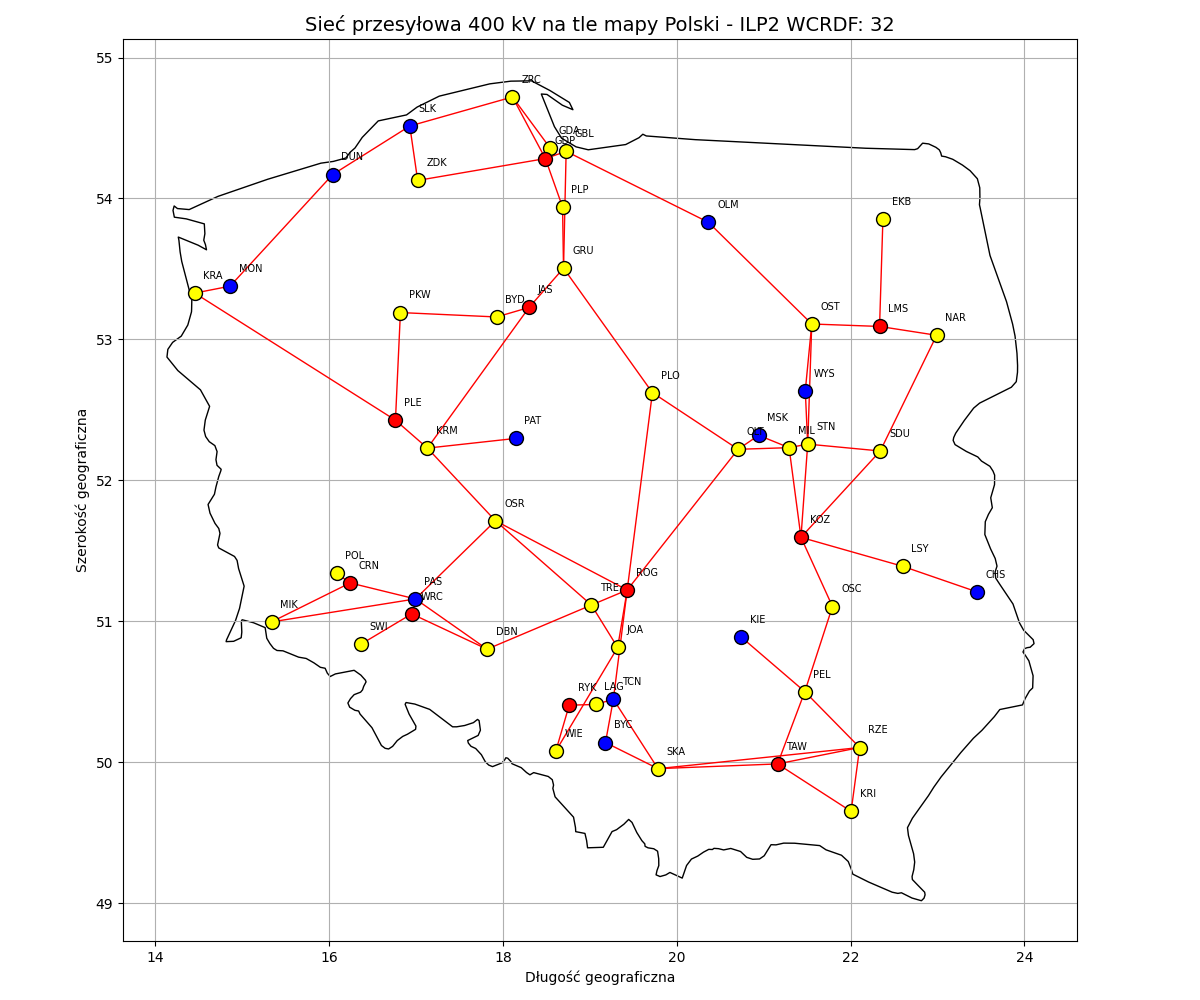
\includegraphics[width=\linewidth]{assets/Poland/img.png}}
    \end{subcaptionbox}
    \hfill
    \begin{subcaptionbox}{Greedy\label{fig:img2}}[0.48\linewidth]
        {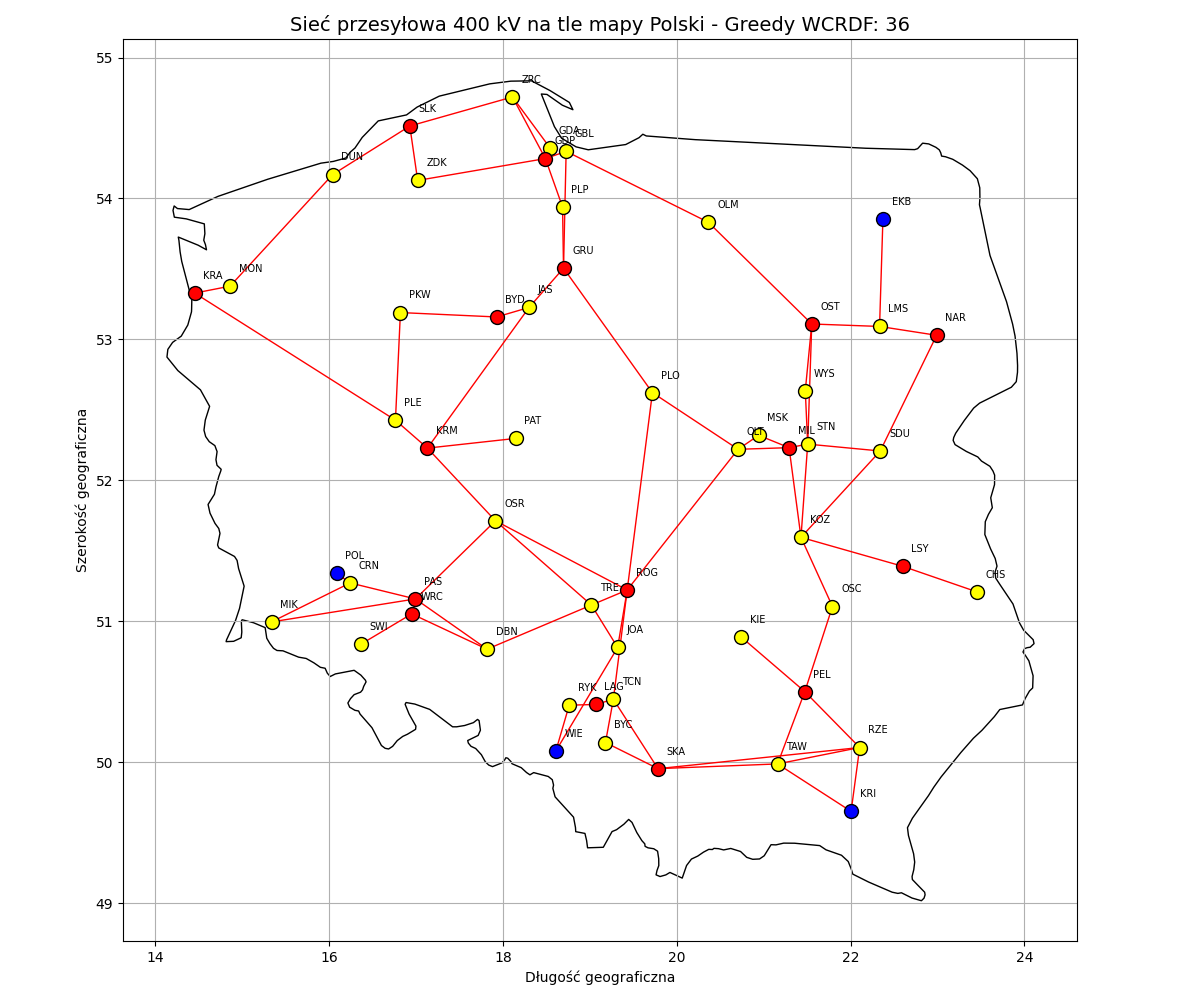
\includegraphics[width=\linewidth]{assets/Poland/img_2.png}}
    \end{subcaptionbox}
    \hfill
    \begin{subcaptionbox}{Approx\label{fig:img1}}[0.48\linewidth]
        {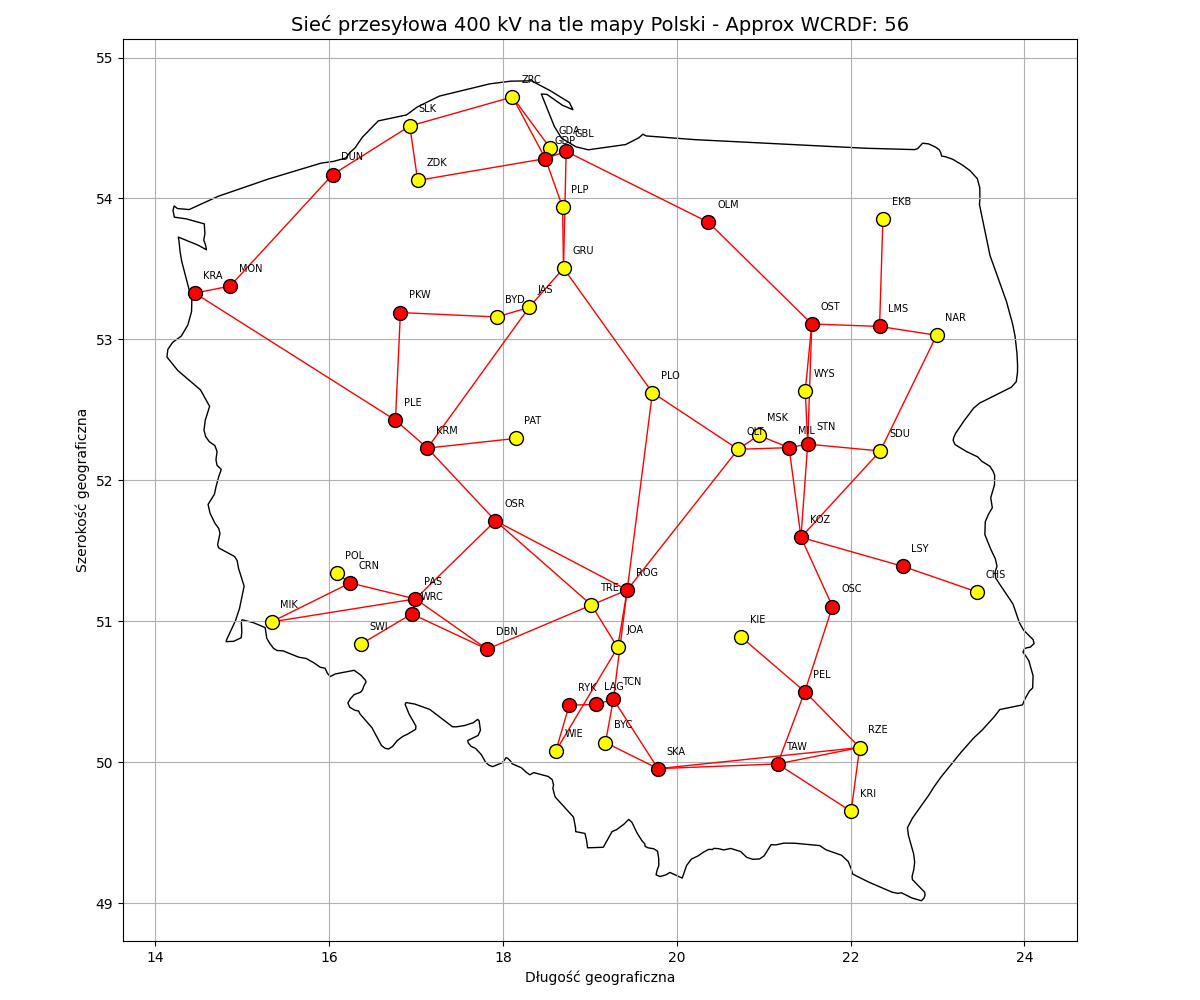
\includegraphics[width=\linewidth]{assets/Poland/img_1.png}}
    \end{subcaptionbox}
    \caption{Efekt działania algorytmów ILP, Greedy i Approx dla problemu rozmieszczenia zabezpieczeń sieci energetycznych.}
    \label{fig:poland}
\end{figure}

\begin{table}[H]
    \centering
    \begin{tabular}{|c|c|c|}
        \hline
    Algorytm & WCRDF & Czas działania [s] \\     \hline
    ILP2 & 32 & 2,7014378 \\ \hline
    Greedy & 36 & 0,0003222 \\ \hline
Approx & 56 & 647,6564676 \\ \hline
\end{tabular}
\caption{Wynik działania wybranych algorytmów dla problemu rozmieszczenia zabezpieczeń sieci energetycznych.}
\end{table}

\section{Rozmieszczenie agentów wykrywających oszustwa w internetowej sieci społecznościowej}

\begin{figure}[htbp]
    \centering
    \begin{subcaptionbox}{ILP, WCRDF: 7\label{fig:ilp}}[0.48\linewidth]
        {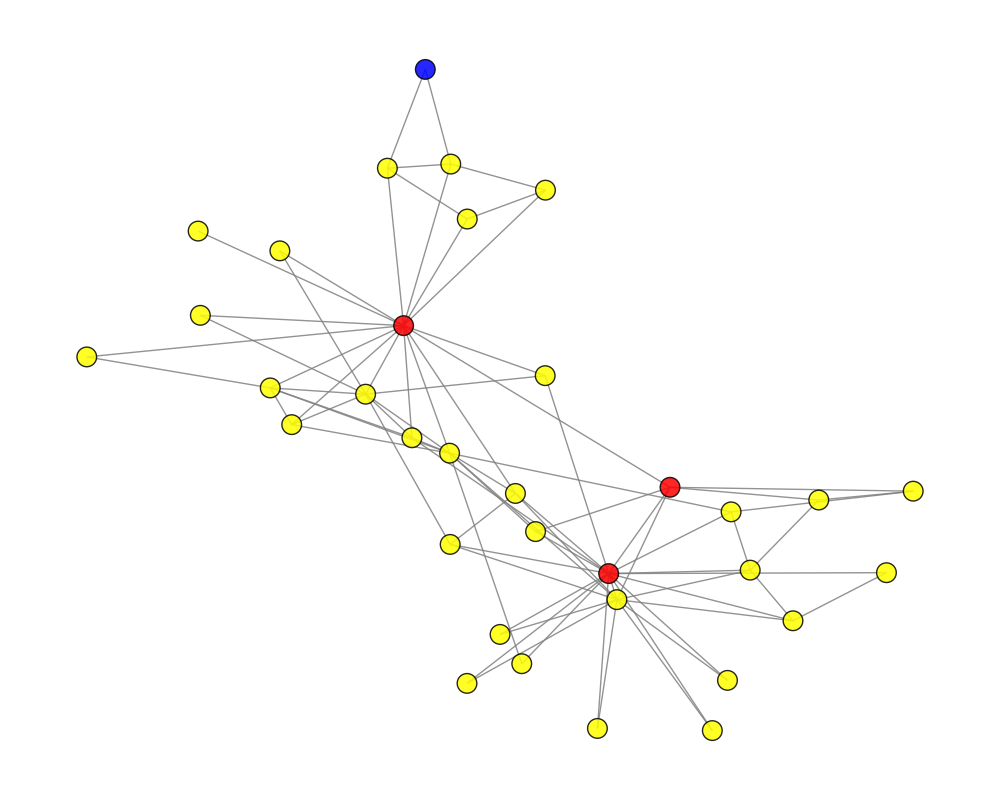
\includegraphics[width=\linewidth]{assets/Facebook/ilp.png}}
    \end{subcaptionbox}
    \hfill
    \begin{subcaptionbox}{ILP2,  WCRDF: 7\label{fig:ilp2}}[0.48\linewidth]
        {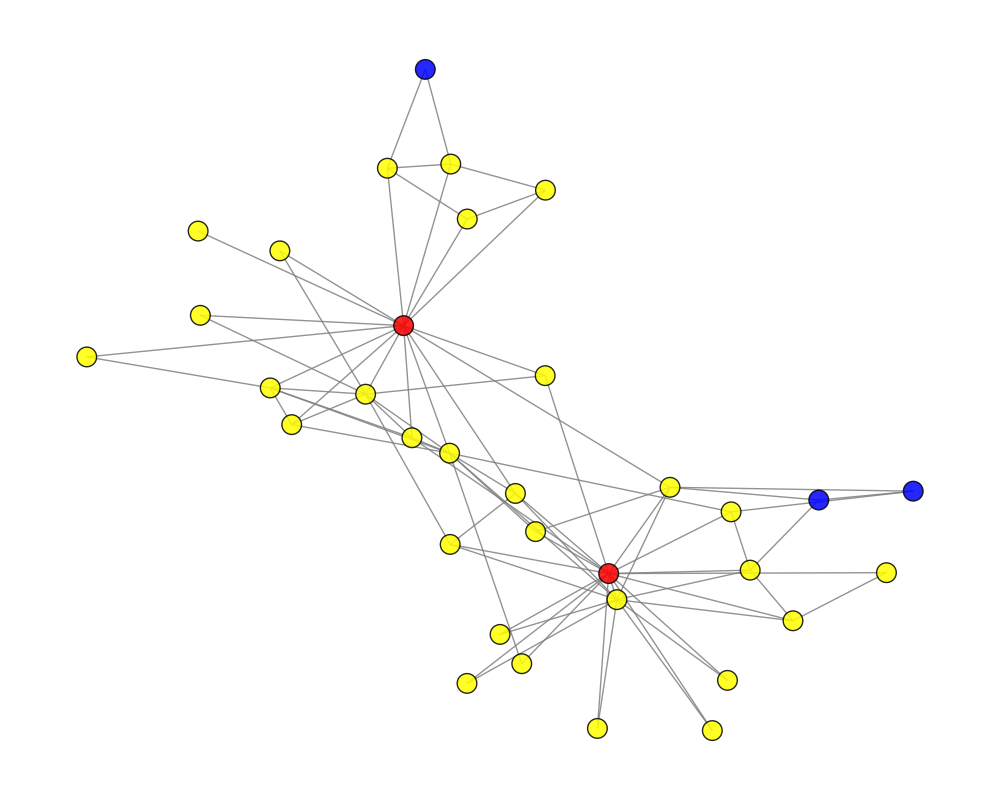
\includegraphics[width=\linewidth]{assets/Facebook/ilp2.png}}
    \end{subcaptionbox}
    \hfill
    \begin{subcaptionbox}{Greedy  WCRDF: 7\label{fig:greedy}}[0.48\linewidth]
        {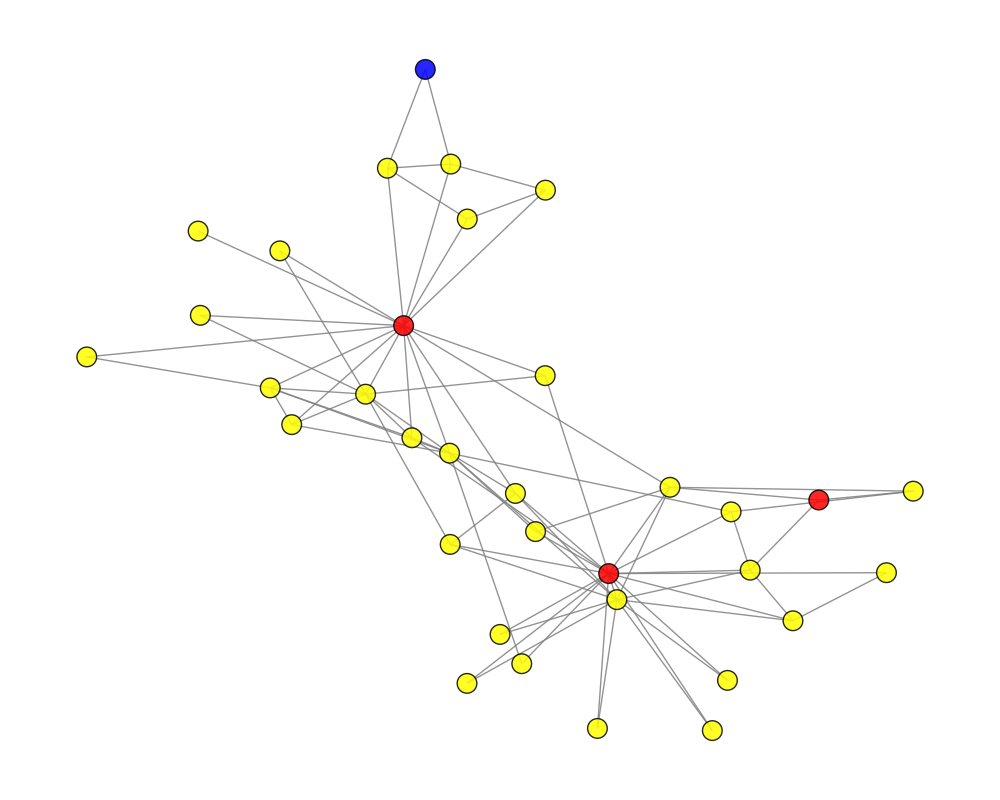
\includegraphics[width=\linewidth]{assets/Facebook/greedy.png}}
    \end{subcaptionbox}
    \hfill
    \begin{subcaptionbox}{Approx  WCRDF: 8\label{fig:approx}}[0.48\linewidth]
        {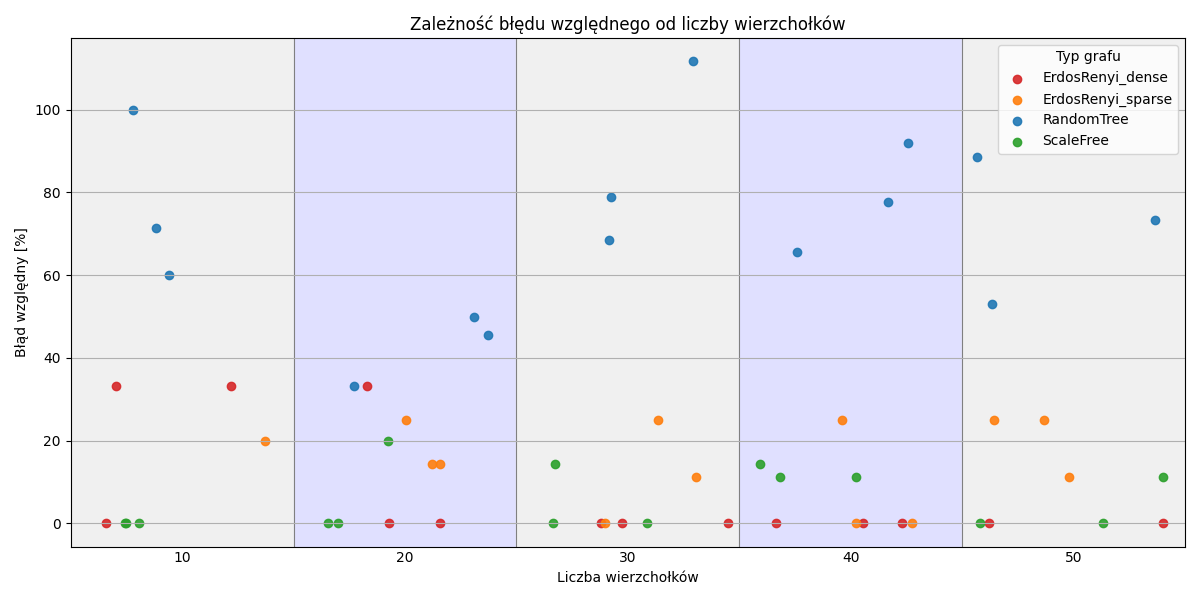
\includegraphics[width=\linewidth]{assets/Facebook/approx.png}}
    \end{subcaptionbox}
    \hfill
    \begin{subcaptionbox}{AntColony  WCRDF: 21\label{fig:ant}}[0.48\linewidth]
        {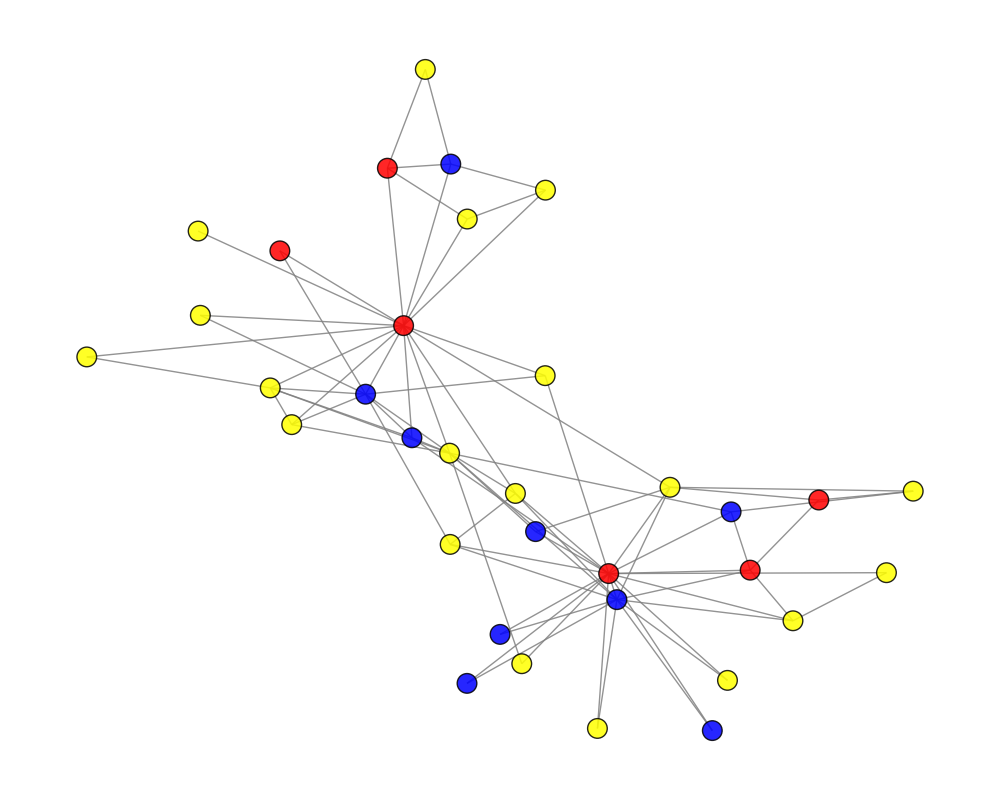
\includegraphics[width=\linewidth]{assets/Facebook/ant.png}}
    \end{subcaptionbox}

    \caption{Efekt działania algorytmów ILP, Greedy i Approx dla problemu rozmieszczenia agentów w małej, rzeczywistej sieci społecznościowej.}
    \label{fig:karate}
\end{figure}

\begin{table}[H]
    \centering
    \begin{tabular}{|c|c|c|}
        \hline
    Algorytm & WCRDF & Czas działania [s] \\     \hline
    ILP2 & 7 & 0,0865662 \\ \hline
    ILP & 7 & 0,0624058 \\ \hline
    Greedy & 7 & 0,0001245 \\ \hline
    Approx & 8 & 0,1533187 \\ \hline 
    AntColony & 21 & 5,1319121 \\ \hline
\end{tabular}
\caption{Wynik działania wybranych algorytmów dla problemu rozmieszczenia agentów w małej sieci społecznościowej.}
\end{table}

\begin{figure}[H]
    \centering
    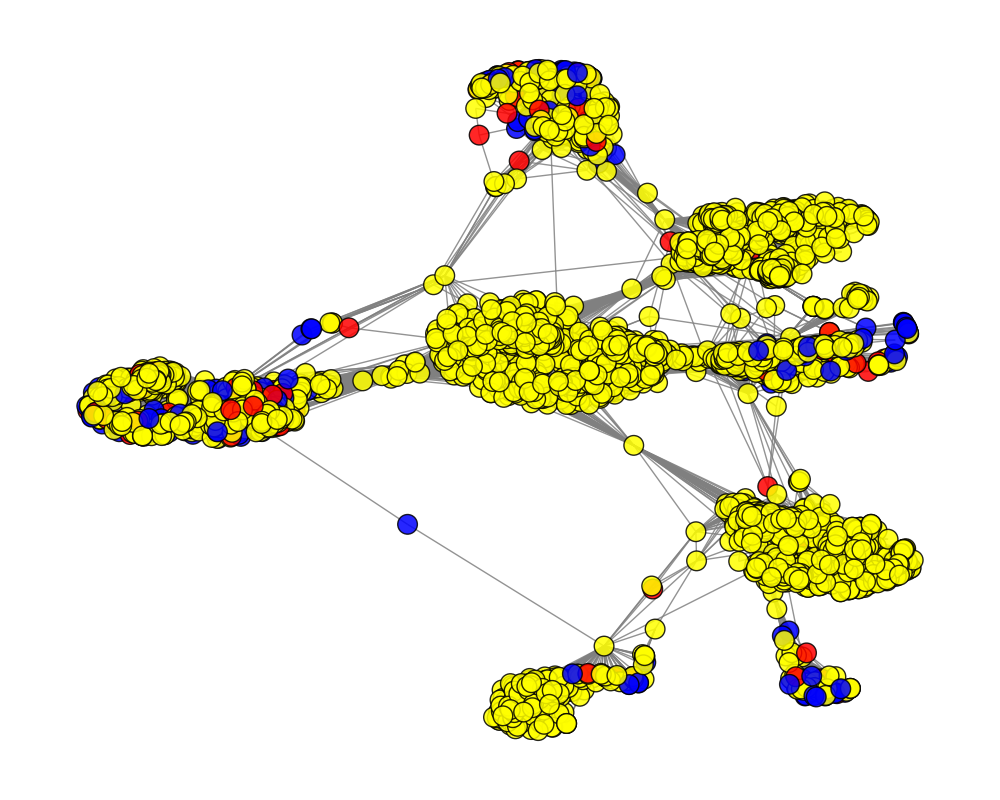
\includegraphics[width=0.75\textwidth]{assets/Facebook/facebookgreedy.png}
    \caption{Efekt działania algorytmu zachłannego dla problemu rozmieszczenia agentów w dużej, rzeczywistej sieci społecznościowej. WCRDF: 411, czas działania 2,9348995 s.}
    \label{fig:fbgreedy}
\end{figure}